\documentclass{article}

\usepackage{graphicx}
\usepackage{array}
\usepackage[group-separator={,}]{siunitx}
\usepackage{authblk}	% prettier multiple authors

\title{Real Time Social Data Sampling }
\author[]{Scott Hendrickson}
\author[]{Brian Lehman}
\author[]{Joshua Montague}
\affil[]{ \Large{Gnip, Inc.} }

\begin{document}
\maketitle

%%%%%%%%%%%%%%%%%%%%%%%%%%%%%%%%%%%%%%%%%%%%%%%%%%%%%%%%%%%%%%%%%%%
\section{Introduction}

We often wish to calculate social activity rates to identify signals of emerging topics or stories.
And we want to what we can detect and understand the certainty in our estimates.  Ultimately, we want to design for a given level of certainty and signal sensitivity.

This means we need to calculate the relationship between activity counts, observation time, signal sensitivity and confidence. This is illustrated in Figure~\ref{fig:tradeoff}. The event rate is the number of activities per time, the signal is the change in rate, and confidence comes from the statistics of the activities and sampling operators.

%%%%%
% figure
%
\begin{figure}[h]
    	%\centering
	\begin{center}
		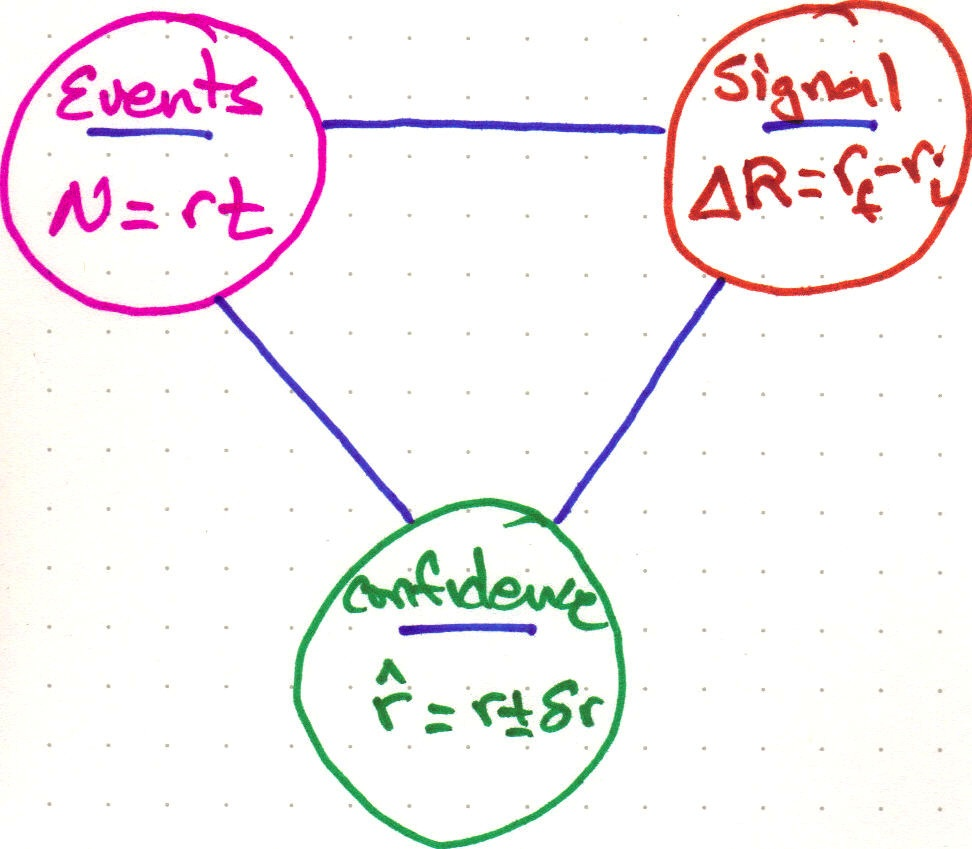
\includegraphics[width=1.75in]{./imgs/tradeoff.jpg}
	\end{center}
	\caption{The number of events is a product of the rate and time. Signal is the change in event rate we want to detect.  Confidence is the way to characterize the uncertainty in our estimate of rate. These parameters are not independent: choose any two and calculate the third. }
    	\label{fig:tradeoff}
\end{figure}
%
%
%%%%%

For many topics, social media streams contain data with significant enough volume and frequency to create reliable, high-resolution signals in the time series in short observation times.  But for the less common topics, the activities (e.g. blog posts on curling) are less frequent and we need to take care in identifying the observation time, signal sensitivity and confidence level. These three quantities are related; typically, we can choose two and the third will be defined for the stream we are watching.

There are a handful of related questions you that may come up around sampling and signals.  In the next section, we list some of these questions. In the following section, we will look at filtering and sample in a little more detail.  The middle of this white paper builds up the calculation method required to answer these questions. Finally, we provide some example calculations.

%%%%%%%%%%%%%%%%%%%%%%%%%%%%%%%%%%
\subsection{Motivating Questions} 

Common questions around rate estimates, signal and confidence level:

\begin{itemize}
\item I plan to bucket the data in order to estimate activity rate, how big (i.e. what duration) should the buckets be? 
\item How many activities should I target to collect in each bucket in order to be have a 95\% confidence that my rate estimate is accurate? 
\item The activity rate has doubled from five counts to ten counts between two of my buckets. Is this a significant change? Or is this expected variation due to low-frequency events?
\item I want to minimize the total number activities I consume, what sampling factor should I use if I want to detect changes of 2x in activity rate in 1-hour?
\item How many buckets do I aggregate to optimize the trade-off between signal sensitivity and signal latency?
\item How do I describe the trade-off between signal latency (how long I have to wait) and rate uncertainty (how confidently I can estimate activity rate)?
\item How do I define confidence levels on rate estimates for a social activity time series with only 20 events per day?
%\item \ldots
\end{itemize}

%%%%%%%%%%%%%%%%%%%%%%%%%%%%%%%%%%
\subsection{Sample Operators and Order of Filters} 

An additional complexity is that you may also choose to sample a known fraction of the total social activities to control costs or to scale analysis.  
This effectively decreases the rate of activities. It may be useful to take a detour into sampling before moving the the core 
of the calculation.  If not, just skip to the next section.

There are two approaches to sampling a firehose of social data. Both involve reducing the number of activities in the real time stream to an
intermediate, manageable size for analysis.

The first step is to use keyword filtering.  Gnip provides filtering on keywords to select only the portion of the stream that is relevant to the topic you want to analyze. For example, if you are interested in tracking the Super Bowl, you might start with a broad stream defined by the keywords ``superbowl" ``super~bowl" and ``contains:xlvii", the latter being the Roman numeral of the Super Bowl as might be seen in hashtags or short links. This would limit the social data stream to activities related to the Super Bowl.

In the case of a major event like the Super Bowl, the keyword-filtered stream may represent a very large number of activities.  In this case, a second step might be to filter this stream to a known fraction of the total firehose. For example, using Gnip's sampling operator, we can reduce the stream to only fraction, e.g. 12\%, of the activities. The corresponding Powertrack rule would become  ``(super bowl OR superbowl) sample:12''.

It is useful to know how Gnip's sampling algorithms work to inform sampling decisions.  Sampling is available on Gnip's premium streams including Tumblr, Twitter, Wordpress and Disqus. Some key features of Gnip sampling :

\begin{enumerate}
	\item 1\% resolution
	\item Effective sampling rate stable (short time resolution)
	\item Sample is deterministic and returns the same activites for near-rule matches.  For example, this means that you will get the same tweets for matches to the ``super bowl'' portion of the rules ``super bowl sample:12'' and ``(super bowl OR superbowl) sample:12''
	\item Progressively inclusive (i.e. the 2\% stream includes the activities from the 1\% stream plus an additional 1\%,  and so on)
	\item Activities are first selected from the firehose to reach the desired sampling rate and then filtered by keywords 
\end{enumerate}

What happens when we look at the combination of filtering with sampling?  Continuing with our Super Bowl example, assume our term filtering rules return $y=5\%$ of the stream. Assume further that we sample $x=12\%$ sample of the firehose activities and thee total activities for the day are $N_f=500$M.
Filtering and sampling will leave us with approximately,

\begin{equation}
    \label{eq:sbsample}
    N_{obs} = x y N_f = 0.12 (0.05) 500 \textrm{M = 3M}
\end{equation}
observed activities in a day. 

Once you understand this order, it is natural to ask why Gnip does not filter first, then sample. The difference is not in the final outcome, but how long you have to wait for a reliable estimate of rate. If Gnip were to filter on keywords first, followed by sampling, Equation~\ref{eq:sbsample} would also be a reasonable estimate of $N_{obs}$ on the time scale of the sampling calculation. However, this process would require relaxing properties 3 and 4 in the list above. Both attributes are desirable for most social data projects. Doing the sample first, followed by the keyword filter, gives a slightly more complex behavior because it amplifies the effects of statistical variations in the short term.

%%%%%%%%%%%%%%%%%%%%%%%%%%%%%%%%%%%%%%%%%%%%%%%%%%%%%%%%%%%%%%%%%%%
\section{Signal} 

In many situations, the main question is: \emph{``How many events must we observe in order to detect a signal?"} Answering this question requires an understanding of the trade offs between sampling time, activity rates, and signal size.  First, we will define signal in terms of the activity rate.

%%%%%%%%%%%%%%%%%%%%%%%%%%%%%%%%%%
\subsection{Activity Rate} 

The activity rate is calculated by,

\begin{equation}
    \label{eq:rateEst}
    \bar{r} = \frac{N}{T}
\end{equation}
where $N$ is the number of activities and $T$ the time period over which we count.  Because there will be statistical variations in the number of activities we count in any given time interval, there will be some uncertainty in our estimate of average rate. The more activities we count, the lower the uncertainty in our estimate.

%%%%%
% figure
%
\begin{figure}[h]
	\begin{center}
		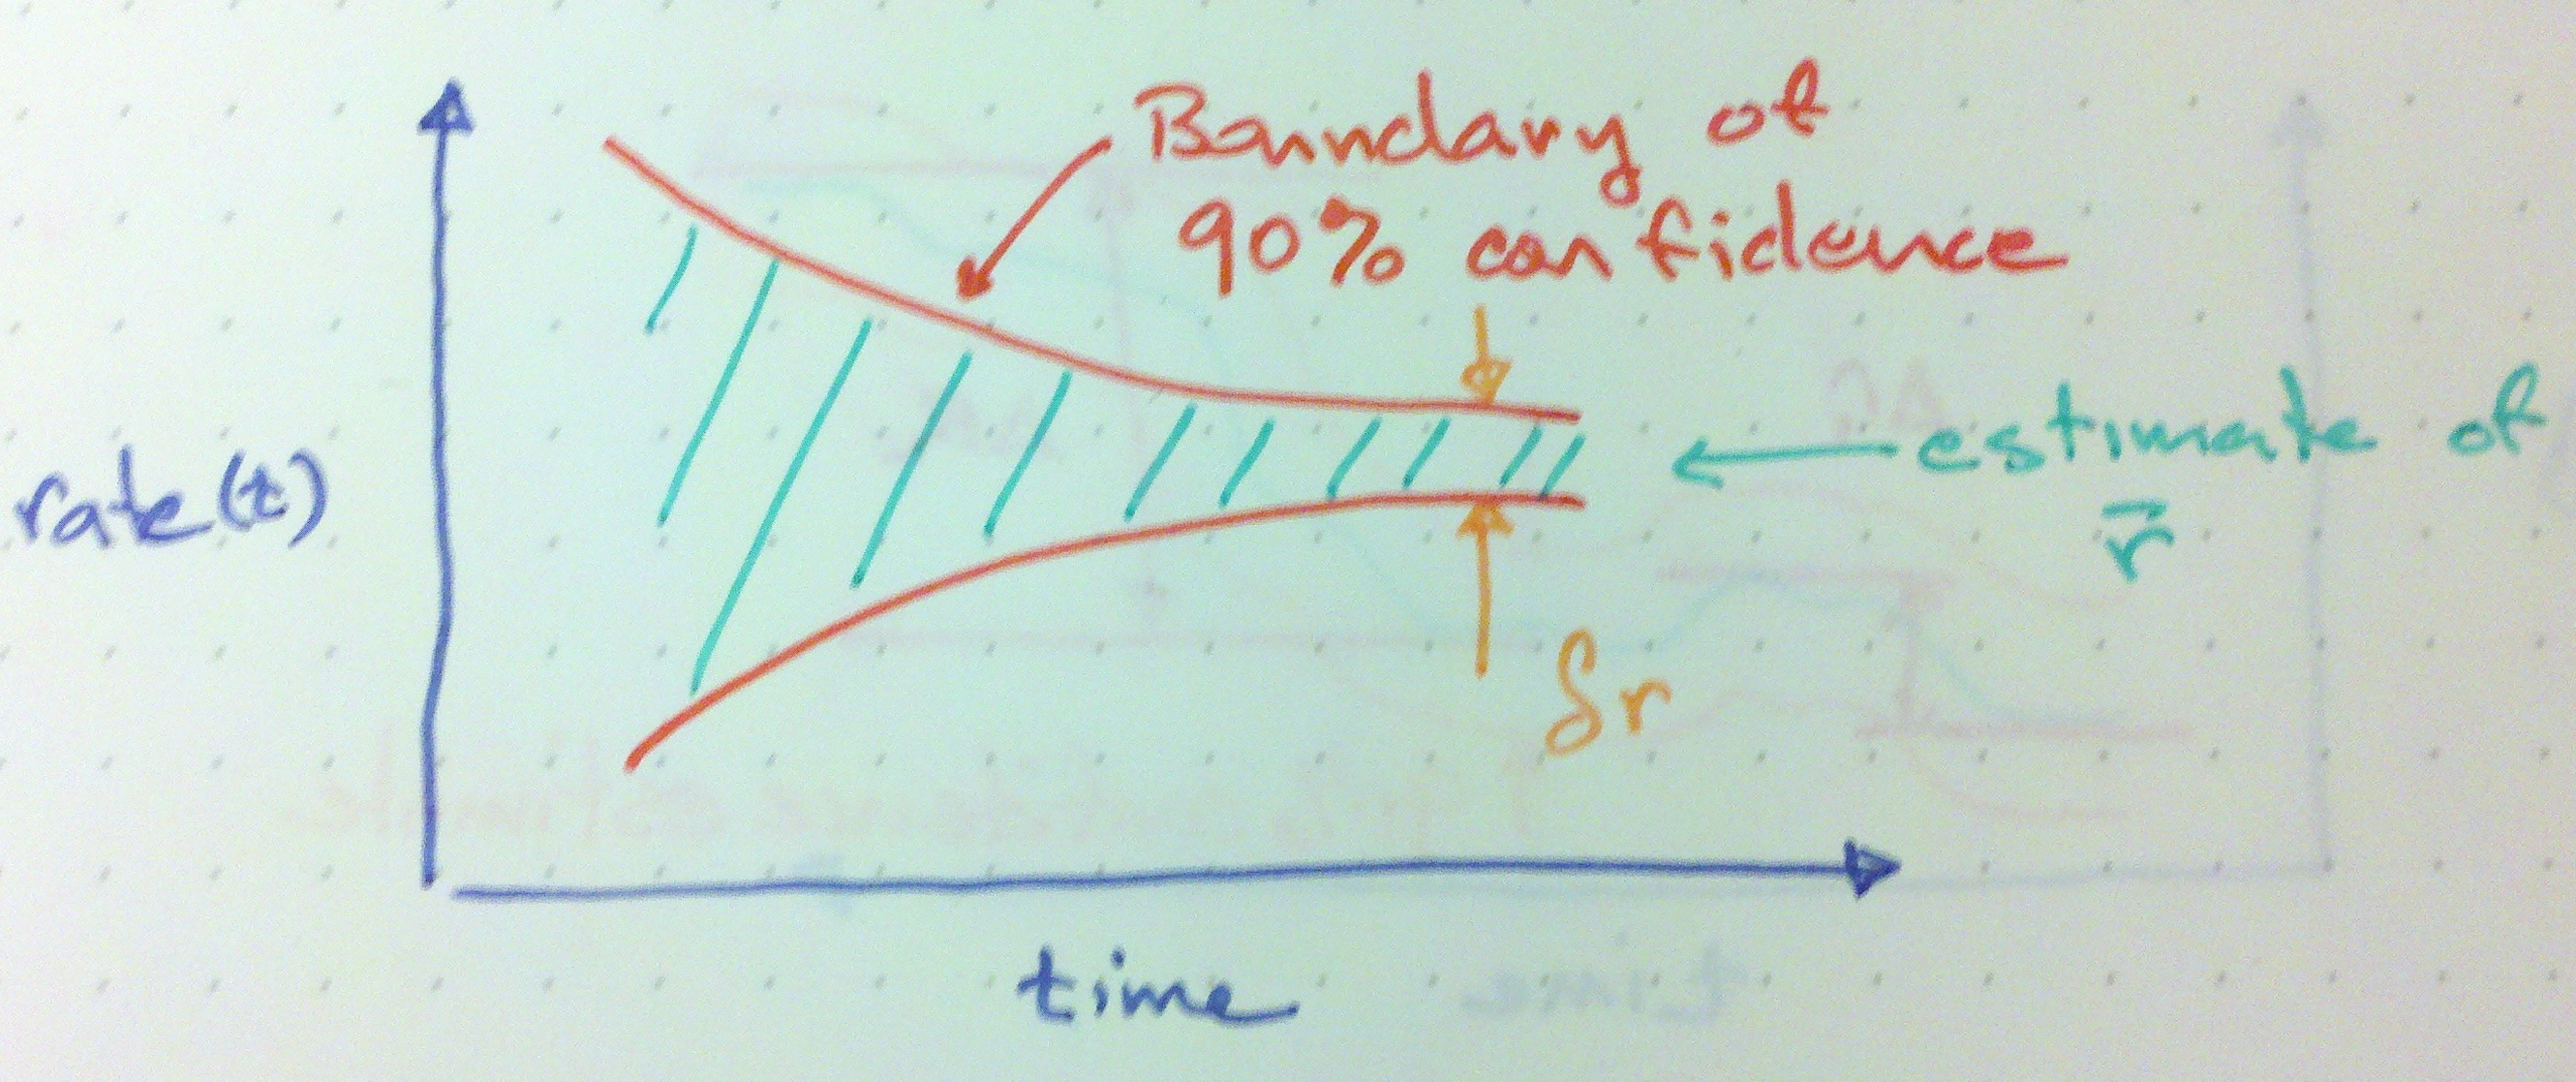
\includegraphics[width=4.0in]{./imgs/confidence.jpg}
	\end{center}
	\caption{Uncertainty in the estimated rate of activities goes down as we observe more events. }
    	\label{fig:confidence}
\end{figure}
%
%
%%%%%

Below, we will determine how many activities $N$ we need to count to estimate the average activity rate, $\bar{r}$, to a desired level
of confidence (e.g. 95\%). Or inverting this question: given a level of confidence, how wide is the range of uncertainty
about the rate estimate?  This is a useful framing of the question because we are often trying to detect changes on activity
rate. This is as our signal. 

The details of calculating the confidence level can be found in the next section.  Frist, we explore the connection between
uncertainty in the rate estimate and the size of the signal we can detect.

%%%%%%%%%%%%%%%%%%%%%%%%%%%%%%%%%%
\subsection{Signal Sensitivity}

When activity rates are high, rate estimates will be more certain; when low, rate estimates will be less certain. High uncertainty
in the rate estimates may hide small changes in activity rates we wish to identify.  The variation in activity rate do to infrequent
events or sort time observations must be smaller than the signal we want to detect. Therefore, we observe a valid signal in a time
series when the activity rate has changed by more than the rate Signal Sensitivity, $\Delta r$, defined as,

\begin{equation}
    \label{eq:signal}
    | r(t_f) - r(t_i) | \geq \Delta r.
\end{equation}

The associated time scale of the change, $T_l = t_f - t_i$, is the Signal Latency.  This definition implies that the we must observe activities for a time $T > T_l$ to achieve Signal Sensitivity $\Delta r$.

%%%%%
% figure
%
\begin{figure}[h]
    \centering
    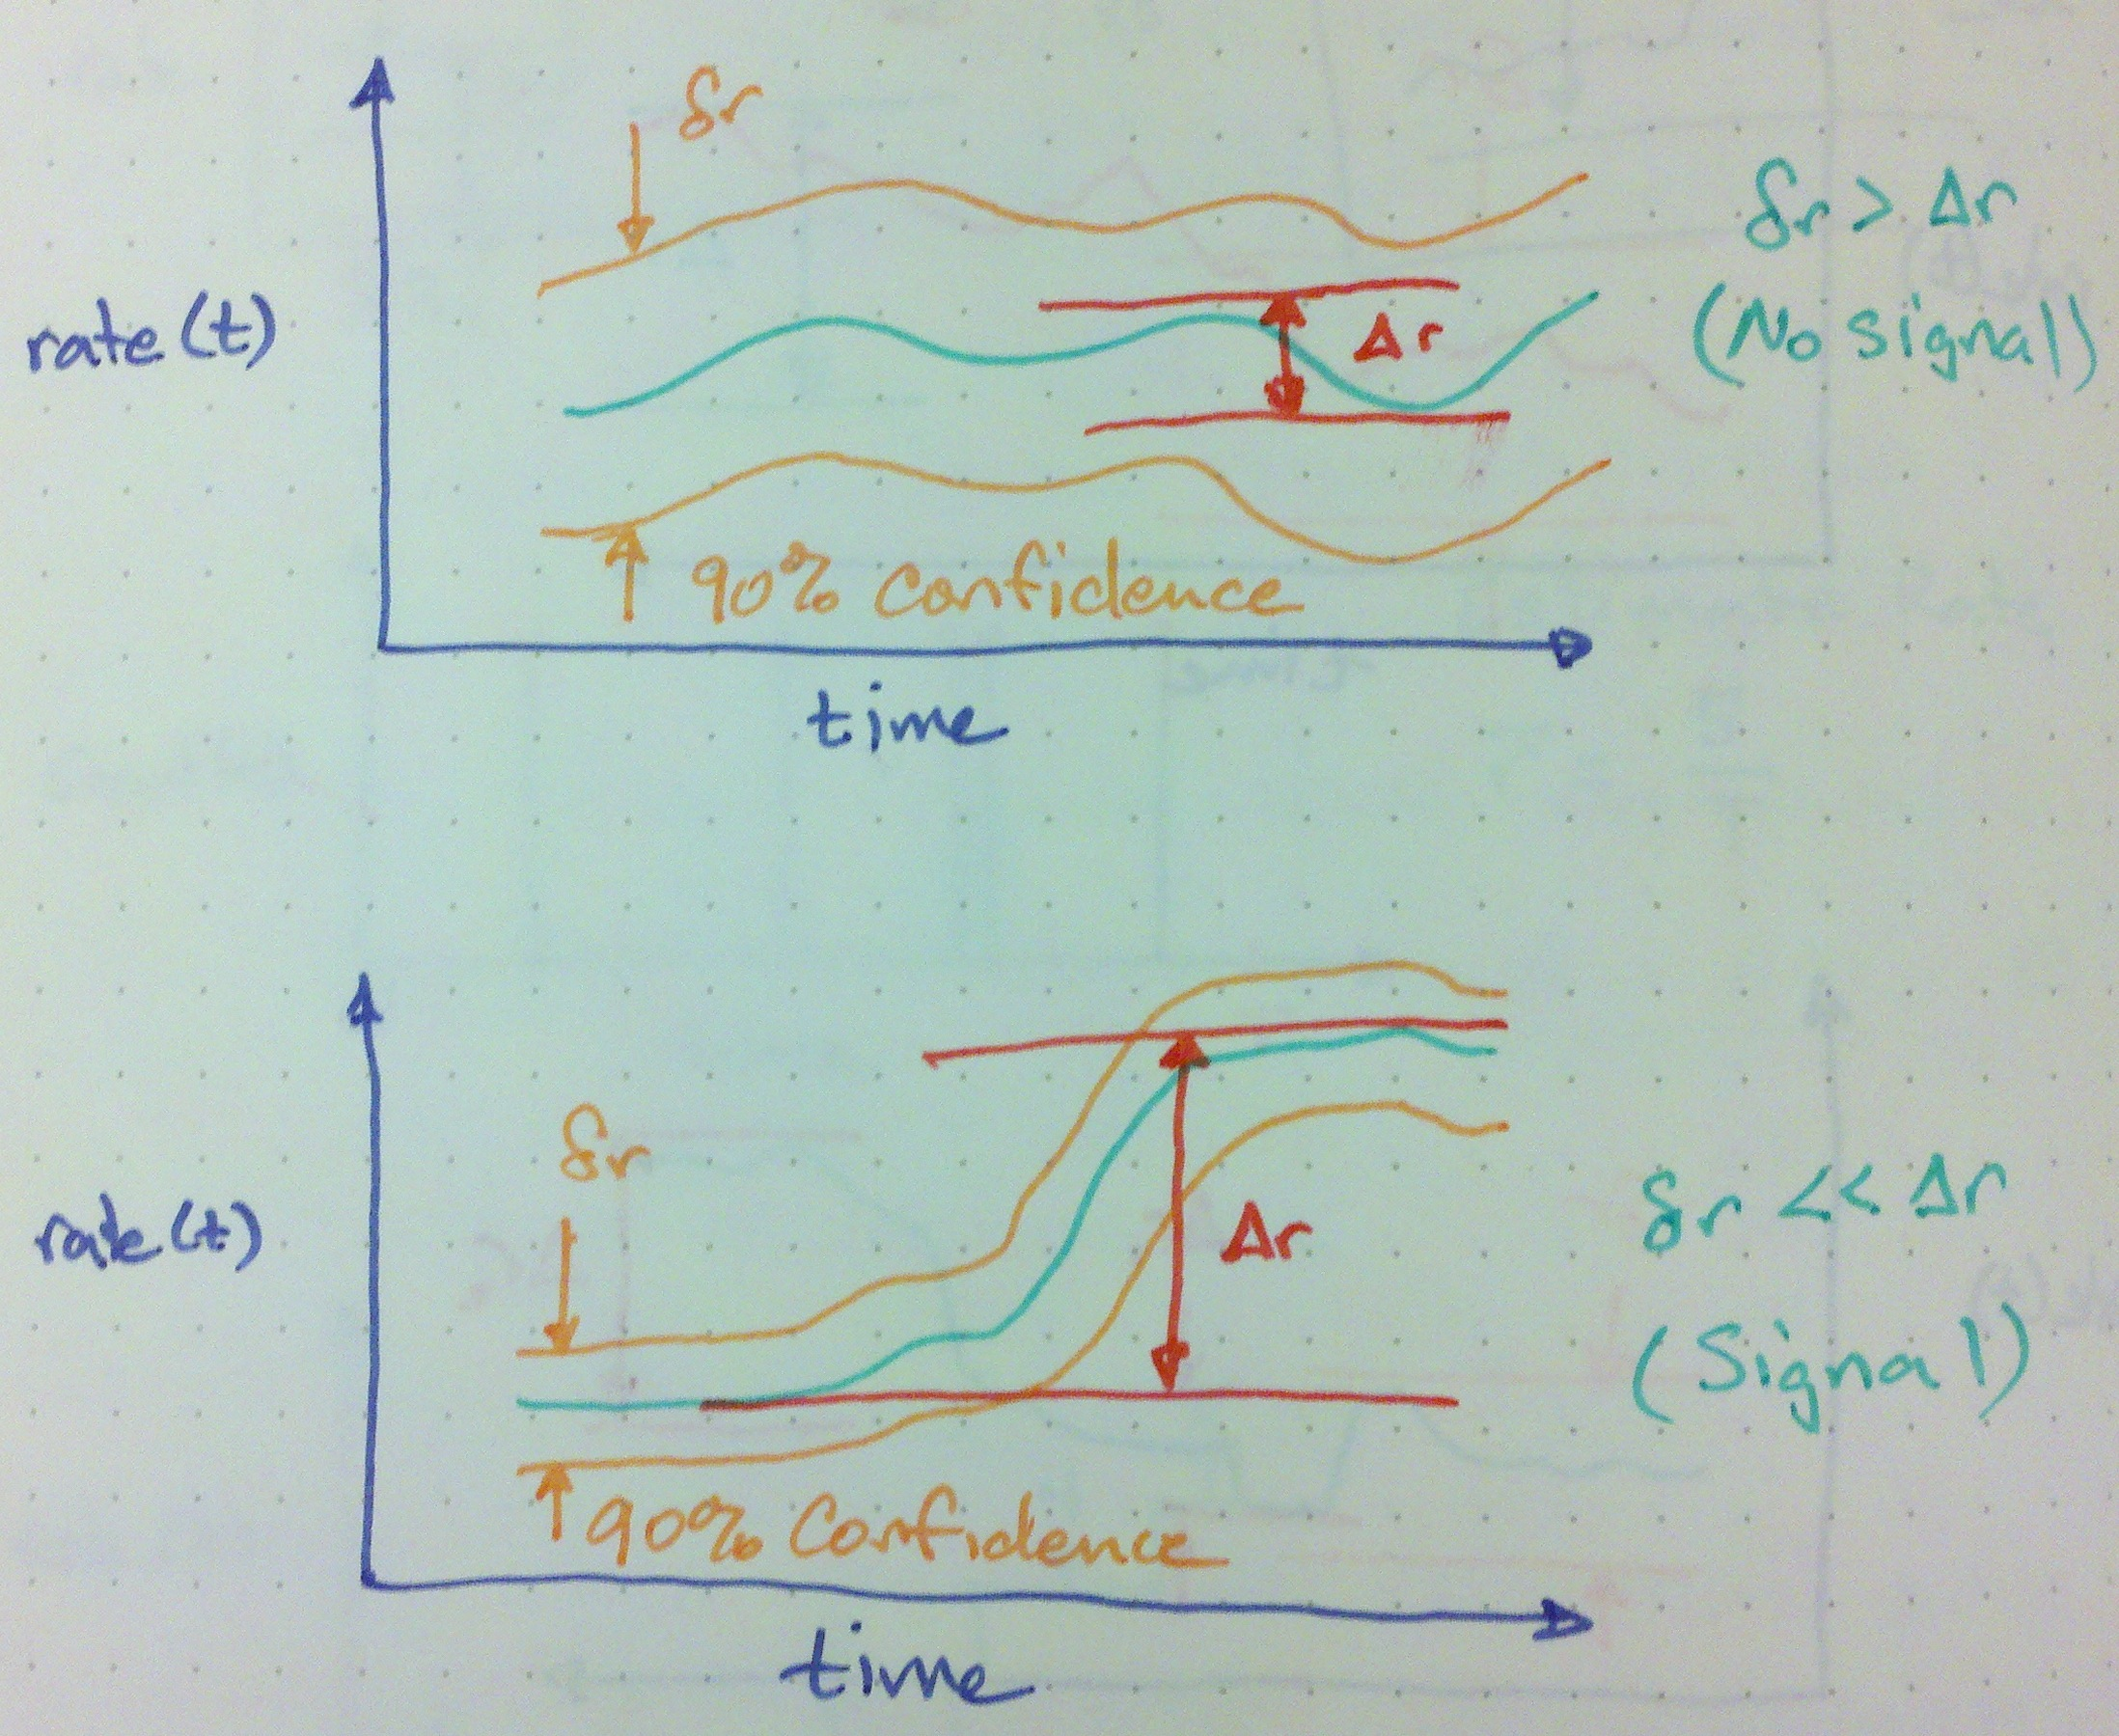
\includegraphics[width=3.5in]{./imgs/signal.jpg}
        \caption{A signal can be detected when the change in rate is greater than the uncertainty in the rate estimates.}
    \label{fig:signal}
\end{figure}
%
%
%%%%%

%%%%%%%%%%%%%%%%%%%%%%%%%%%%%%%%%%
\subsection{Signal Sensitivity--Confidence Criteria} 

We will be estimating the activity rate in Equation~\ref{eq:rateEst} by counting activities for a determined time period.  The
number of counts in any given period will be distributed about the long term mean. As we count more activities, our
estimate of rate will converge to the true value.  If we count thousands of activities per minute, our confidence of the estimate
of activity rate will be very high after a short time.  For rare activities, we will have to count for a longer time before we have
a high level of confidence in our rate estimate.

Referring to the Signal Sensitivity definition in Equation~\ref{eq:signal}, we can establish a rough criteria for confidence
in terms of signal uncertainty, $\delta r$:

\begin{equation}
    \label{eq:criteria}
    \frac{\delta r}{\bar{r}_{max}} << \frac{\Delta r}{\bar{r}_{max}}.
\end{equation}
where $\bar{r}_{max}$ will be the lower rate estimate (initial if detecting rising activity rate but final if detecting falling activity rate).

The relative variation of the observed rate from the average rate will decrease with an increasing number events.
To help quantify this inequality, we introduce a criteria factor, $\eta$, that quantifies how much larger than the relative
uncertainty the change in rate must be.

\begin{equation}
    \label{eq:criteriaParam}
    \frac{\delta r}{\bar{r}_{max}} = \frac{\eta \Delta r}{\bar{r}_{max}}
\end{equation}
where $\eta \ge 1$.

This criteria represents trade off between signal size and confidence.

%%%%%%%%%%%%%%%%%%%%%%%%%%%%%%%%%%%%%%%%%%%%%%%%%%%%%%%%%%%%%%%%%%%
\section{Statistics of Time Series of Activities} 

In this section, we examine the underlying statistics in order to calculate confidence intervals and confidence levels.

%%%%%%%%%%%%%%%%%%%%%%%%%%%%%%%%%%
\subsection{Poisson Activity Probability} 

A model of counts of rare activities is that the inter-arrival times are exponentially distributed, 

\begin{equation}
    \label{eq:tbe}
    p_{activity}(t) = r e^{-r t}
\end{equation}

This assumption leads a Poission distribution of activity counts over time.

The probability of observing $n$ activities in time $t$ when the activity rate is $r$ is given by,
\begin{equation}
    \label{eq:poisson}
    P(n) = \frac{e^{-r t} (r t)^n}{n!}
\end{equation}

The expected value is $E[n]=n=rt$. The mean and variance of the Poisson distribution are both equal to $r$.

%%%%%%%%%%%%%%%%%%%%%%%%%%%%%%%%%%
\subsection{Poisson Confidence Intervals} 

We are counting activities in a defined time interval to estimate the activity rate $r$.  Confidence in the estimate of $r$ goes up as we count more and more activities. Confidence intervals for the Poisson distribution with confidence level $1-\alpha$ are given by

\begin{equation}
    \label{eq:chisqconf}
    \frac{1}{2T} \chi^2(\alpha/2;2n) \leq r \leq \frac{1}{2T} \chi^2(1-\alpha/2;2n+2)
\end{equation}
where $\chi^2$ is the inverse cumulative distribution function, $CDF^{-1}(p; n)$, of the $\chi^2$ distribution.\footnote{A useful approximation to the exact interval is given by  $[ n(1 - \frac{1}{9n} - \frac{z_{\alpha}}{3\sqrt{n}})^3 , (n+1)(1- \frac{1}{9(n+1)} + \frac{z_{\alpha}}{3\sqrt{n+1}})^3]$. }
Note that with this definition of $\alpha$, a confidence interval of 90\% corresponds to $\alpha=0.1$.

Confidence interval sizes for confidence levels of 90\% are shown in \ref{tab:conf}

\begin{table}
    \begin{tabular}{r|l|r|r}
     \hline
N & Interval Bounds & Interval Size & Relative Interval\\ 
\hline 
1 &  [ 0.0513, 4.744 ] & 4.693 & 4.693\\ 
2 &  [ 0.3554, 6.296 ] & 5.940 & 2.970\\ 
3 &  [ 0.8177, 7.754 ] & 6.936 & 2.312\\ 
4 &  [ 1.366, 9.154 ] & 7.787 & 1.947\\ 
5 &  [ 1.970, 10.51 ] & 8.543 & 1.709\\ 
6 &  [ 2.613, 11.84 ] & 9.229 & 1.538\\ 
7 &  [ 3.285, 13.15 ] & 9.863 & 1.409\\ 
8 &  [ 3.981, 14.43 ] & 10.45 & 1.307\\ 
9 &  [ 4.695, 15.71 ] & 11.01 & 1.223\\ 
10 &  [ 5.426, 16.96 ] & 11.54 & 1.154\\ 
20 &  [ 13.25, 29.06 ] & 15.81 & 0.7904\\ 
30 & [ 21.59, 40.69 ] & 19.10 & 0.6366\\ 
40 & [ 30.20, 52.07 ] & 21.87 & 0.5468\\ 
50 & [ 38.96, 63.29 ] & 24.32 & 0.4864\\ 
60 & [ 47.85, 74.39 ] & 26.54 & 0.4423\\ 
70 & [ 56.83, 85.40 ] & 28.57 & 0.4082\\ 
80 & [ 65.88, 96.35 ] & 30.47 & 0.3809\\ 
90 & [ 74.98, 107.2 ] & 32.25 & 0.3584\\ 
100 & [ 84.14, 118.1 ] & 33.94 & 0.3394\\ 
200 & [ 177.3, 224.9 ] & 47.55 & 0.2378\\ 
300 & [ 272.1, 330.1 ] & 58.00 & 0.1933\\ 
400 & [ 367.7, 434.5 ] & 66.82 & 0.1670\\ 
500 & [ 463.8, 538.4 ] & 74.58 & 0.1492\\ 
750 & [ 705.5, 796.6 ] & 91.11 & 0.1215\\ 
1000 & [ 948.6,  1054. ] & 105.0 & 0.1050\\ 
\end{tabular}
\caption{Confidence intervals given the number of events counted $N$ in unit time $T$.  Rate confidence range is $\delta N/T$.}
\label{tab:conf}
\end{table}
% \delta N (table caption) should be defined somewhere.

To determine the parameters of our data collection system, we find the value of $n$ for which the time interval and confidence level match our requirements.  That is, we can now calculate any one of Signal Sensitivity, Signal Latency, activity rate, and confidence level given all of the other parameters. Calculations for various design choices are illustrated in the last section of this paper.

%%%%%%%%%%%%%%%%%%%%%%%%%%%%%%%%%%
\subsection{Confidence Interval Approximations and Bucketed Activity Counts}

This section deals with approximations to the Poisson confidenc interval for large numbers of actvities and has some observations about bucketed activity counts. You can skip this section and move to calculations in many cases.


\subsubsection{Less-Rare Activities} 

When we observe large numbers of activities, the confidence interval can be estimated using the Normal approximation. For example, for $95\%$ confidence interval the interval is symmetric about the mean and given by,

\begin{equation}
    \label{eq:largenconf}
    \bar{r} - 1.95 \sqrt{\bar{r}/n} \leq \hat{r} \leq \bar{r} + 1.95 \sqrt{\bar{r}/n}
\end{equation}

\subsubsection{Bucketed Activity Counts}

For many reasons, counts may be collected in buckets of some pre-defined time length.  The rate information may by more naturally calculated by bucket rather than the total time $T$ required by our confidence requirements. In general, define the relationship between $T$ and the bucket size (constant) as,

\begin{equation}
    \label{eq:bucket}
    \Delta t = \frac{T}{k}
\end{equation}
where $k$ is the number of buckets that we need to aggregate to observe for time $T$. This parameter can be used to calculate a corresponding signal latency, $k_l = T_l/\Delta t$.

Resolution times are interchangeable with number of buckets $k$ given $\Delta t << T$.  In general, the
bucket resolution time will not be an even multiple of the bucket size.  In this case, imposing the calculation of average rate per bucket $\bar{r} = n/\Delta t$ adds another layer of variability.

%%%%%%%%%%%%%%%%%%%%%%%%%%%%%%%%%%
\subsection{Summary of Parameters and Trade offs}

When activities are common, we can estimate the activity rate to a high level of certainty in a short time. With lower
uncertainty in our estimate of activity rate, we can detect small changes in activity rate--we have high Signal
Sensitivity. For rare activities, we have to wait longer to count enough activities to estimate the activity rate to
the desired level of confidence to detect a small signal. These trade offs are summarized in the Table~\ref{tab:tradeoff}.

For reference, we assemble the parameter definitions and a table summarizing trade off in this section before moving
into the details of calculating confidence intervals for rare events in the next section.  Table~\ref{tab:summary}
summarizes the parameters of the model. Table~\ref{tab:tradeoff} summarizes the trade offs in parameters for
a given target.

\begin{table} [!h]
    \begin{tabular}{m{4cm}| m{7cm}}
     \hline
Parameter  & Definition \\
\hline	
$N$ & Number of activities in time $T$\\
$T$ & Duration of observation\\
$r$ & Activity rate \\
$\bar{r} = N/T$ & Estimate of average activity rate \\
$\delta r$ & Uncertainty of rate estimate \\
$\alpha$ & Confidence\\
$\Delta r$ & Signal Sensitivity: Change in activity rate \\
$T_l$ & Signal latency, time to detect $\Delta r$  \\
$\eta$ & Rate signal criteria factor \\
$\Delta t$ & Bucket size (for bucketed data where $\Delta t <T$) \\
$k$ & Duration in number of  buckets ($k=T/\Delta t$) \\
\hline
\end{tabular}
\caption{Summary of model parameters.}
\label{tab:summary}
\end{table}

\begin{table}[!h]
    \begin{tabular}{ m{4cm}| m{7cm}}
     \hline
Target  & Actions \\
\hline
Minimize Activities  & (decrease $N$)  \\
                                  & increase $\Delta r$ (decrease signal sensitivity)  \\
                                  & decrease confidence (E.g. from 95\% to 90\% )  \\
\hline	
Increase Signal Sensitivity   & (decrease $\Delta r$)  \\
                                  & increase $T$ (increase number of buckets ($k$)  \\
                                  & or increase bucket size ($\Delta t$) )  \\
                                  & increase activity rate ($r$) by broadening filter or increase PowerTrack sampling \\
\hline
Decrease Signal Latency      & (decrease $T_l$)  \\
                                 & decrease signal sensitivity $\Delta r$  \\
                                 & decrease confidence factor ($\alpha$) \\
                                 & increase activity rate ($r$) by broadening filter or increase PowerTrack sampling \\
\hline
Decrease Signal Uncertainty & (decrease $\delta r$ or decrease $\eta$) \\ %decreasing eta will restrict the signal  
                          	 & increase $T$ (increase number of buckets ($k$)  \\
                                 & or increase bucket size ($\Delta t$) )  \\
                                 & increase activity counts (increase $N$, $r$) by broadening filter or increase PowerTrack sampling \\
\hline
\end{tabular}
\caption{Summary of model trade offs.}
\label{tab:tradeoff}

\end{table}

%%%%%%%%%%%%%%%%%%%%%%%%%%%%%%%%%%%%%%%%%%%%%%%%%%%%%%%%%%%%%%%%%%%
\section{Example Calculations} 

We present some example calculations to make this concrete and illustrate the use of the lookup tables.

%%%%%%%%%%%%%%%%%%%%%%%%%%%%%%%%%%
\subsection{Estimate the Optimal Powertrack Sampling Operator Value} 

The Sampling Operator, $S$, is the percent sample size extracted from the firehose.  Selecting $S$ is a process that starts at $S =100\%$.  Carefully monitoring the number of activities, $N$, that are filtered through the rules, we get an estimate for $r$ called $\bar{r}$.  Careful monitoring requires a specific report of $\bar{r}$ over small time periods $T$.

Using 100\% of the firehose for one minute, imagine that we observe $\bar{r}=10$ activities.  Further, say that we want to detect a change in activity rate of 20 activitities per minute using $\eta = \frac{1}{3}$.  What sample size should we extract from the firehose?  

The answer to this question depends latency.  We must observe at least 10 minutes of activities to detect our desired signal (see Estimate Signal Latency for calculation).  Is this latency unnecessarily fast?  The comfort level with latency time is user defined.  

Say instead, we are comfortable with a latency of 2 days.  Given that we expect $\frac{10}{1}$ activites per minute or $14,400$ activities per day, we need to meet our Signal Sensitvity ($\frac{\delta r}{\bar{r}} = \text{ Relative Interval Size} = \frac{1}{3}\frac{(20-10)}{min} \frac{1 min}{10 activities}= 33\%$) over this 2 day period.  Table \ref{tab:conf} requires 100 activies for a $\text{ Relative Interval Size}$ of $33\%$ over this 2 day period.  Hence, instead of using $100\%$ of the firehose, we could use $S = \frac{100}{28,000} << 1\%$.              \ldots

%%%%%%%%%%%%%%%%%%%%%%%%%%%%%%%%%%
\subsection{Estimate Signal Latency} 

% first pass at calc, 2013-04-18, BL

Imagine we observe rate of 10 activities per minute and we want to detect a change in activity rate of 20 activitities per minute.  How long does it take to identify a change in the activity rate as a signal with 90\% confidence level? To calculate an answer, we will be using the Signal Sensitivity--Confidence Criteria, \ref{eq:criteriaParam} and Confidence Interval Sizes from Table \ref{tab:conf}

\begin{itemize}
\item Calculating $T_{l}$
\item Signal criteria factor $\eta=\frac{1}{3}$ -- In this case we choose a criteria that reflects our wish to see fewer false positives.
\item Signal Sensitvity $\frac{\eta \Delta r}{\bar{r}} = \frac{1}{3}\frac{(20-10)}{min} \frac{1 min}{10 activities}= 33\%$
\item Confidence Interval Size at $N =10$ is $11.54$. %Confidence intervals around $\r_bar$ only depend on N. 
\end{itemize}

It is clear that we cannot detect a change in activity rate of 10 activities/minute by measuring for only 1 min.  Notice that our criteria is not fulfilled:
\begin{equation}
    \label{eq:ex2:notmet}
    \frac{\delta r}{\bar{r}} = \frac{(11.54)}{10} \approx 115.4\% \not\le 33\% 
\end{equation}

The time $T_{l}$ that it takes to observe this signal $\Delta r =20$ with signal criteria factor of $\eta=\frac{1}{3}$ depends on the total number of activities $N_t$ that we must observe to have a credible estimate of the activity rate. Because activities are infrequent, we will look up the confidence interval size, synomous to $\delta r$, for small numbers of activities in Table \ref{tab:conf}.  As $N_t$ increases, the relative $90\%$ confidence interval size narrows around the average rate, which can be seen through the decreasing realive interval value in Table \ref{tab:conf}.  We need to find the value for $N_t$.

We can only detect a signal $\Delta r$ when our signal criteria is fulfilled:
\begin{equation}
    \label{eq:ex2:met}
    \frac{\delta r}{\bar{r}} = \text{ Relative Interval Size} = 33\% =  \frac{\eta \Delta r}{\bar{r}}
\end{equation}

You can look up the required Relative Interval Size in Table $\ref{tab:conf}, 100\%/3 = 33\%$ to see that we need to observe at least 100 events on average to reach our criteria. Therefore, $T_l = 10 minutes$ because we will have observed 100 activities in 10 minutes given $r_bar = \frac{10 activities}{1 min}$. That is, we must observe 10 minutes of activities to detect our desired signal.

%How long does it take to identify a change in the activity rate as a signal?
%
%As an example for calculating $T_{l}$, we choose a specific signal $\Delta r = \frac{10}{T}$.  The time $T_{l}$ that it takes to observe this signal $\Delta r$, or equivalently, the number of buckets, $k$, depends the total number of activities $N_t$ that we must observe to have a credible estimate of the activity rate. Because activities are infrequent, we will look up the confidence interval for small numbers of activities this up in Table \ref{tab:conf}.  As $N_t$ increases, the $90\%$ confidence interval length $I$ narrows around the average rate $\delta r$ decreases.  See Equation \ref{...}3??.  We need to find the value for $N$ at which point $\delta r$ has decreased enough to allow us to see our signal $\Delta r = \frac{10}{T}$.  
%
%Choosing $\eta=1$, we see in Table \ref{tab:conf} that for $\Delta r = \frac{10}{T}$, we must have $N\geq7$ causing $I > 10\eta$ in order to observe our signal.  Notice that $N_t=7$ is the point after which we could first observe a signal.  Thus, we say that $T_{l}>T_{N_t}$ defines the time that it takes to observe a signal, which means that signal latency is greater than the amount of time that it takes to collect $N_t$ activities.  Takes 2 periods to get the calculation> have to calculate the rate in the first then the second and compare.
%
%We can decrease $T_{l}$ in several ways.  First, we could try improving the rate at which we achieve $N_t$ by  increasing our PowerTrack sampling.  Otherwise, we could decrease $T_{l}$ as we narrow $I$ through a lower confidence level $(1-\alpha)$.  The lower confidence level tightens $I$ around smaller $N$ allowing the potential signal to become clearer faster, but this goal is accomplished at the cost of decreased confidence.  Another basic option is to simply choose a smaller (larger?) signal size such as $\Delta r = \frac{5}{T}$ from our previous example.  All of these strategies would decrease $T_{l}$.



%%%%%%%%%%%%%%%%%%%%%%%%%%%%%%%%%%
\subsection{Estimate Signal Sensitivity}
% first pass at calc, 2013-03-12, JM

Suppose we would like to determine the magnitude of a signal change needed to 
classify it as significant. As shown in Equation~\ref{eq:criteriaParam}, 
classifying a signal $\Delta r$ as significant depends on the choice of criteria factor 
$\eta$ and the observation parameters that determine the uncertainty $\delta r$. 
Specifically, we will need to choose a criteria factor $\eta$ and confidence level 
$(1-\alpha)$, and our observation will be characterized by total activity count $N$ 
and total time $T$.

%Based on the Poisson confidence intervals in Equation~\ref{eq:chisqconf}, our 
%significant signal must then either be 
%
%\begin{equation}
%	\label{eq:sigSig1}
%\Delta r - \bar{r} > \frac{1}{2} \chi^2(1-\alpha/2;2N+2), 
%\end{equation}
%or lower than 
%
%\begin{equation}
%	\label{eq:sigSig2}
%\bar{r} - \Delta r < \frac{1}{2} \chi^2(\alpha/2;2N). 
%\end{equation}


Let us assume we have decided to classify as significant a signal with $\eta = \frac{1}{10}$, or 
$\delta r = \frac{1}{10}\Delta r$. Furthermore, we have chosen a 90\% confidence interval 
($\alpha = 0.1$), and observed $N$=10,000 activities over a period of $T$=1 minute 
(60 seconds) for an estimated activity rate of $\bar r = 167~\si{\per\second}$. We next use 
Equation~\ref{eq:chisqconf} to calculate the interval of activities for our 
90\% confidence level, and divide by observation period $T$ to obtain the corresponding 
minimum significant activity rate $\delta r = 5~\si{\per\second}$. Recall, however, 
that we have also specified a criteria factor $\eta = 10$. Therefore, in this example, 
in order to classify the change in rate as significant, we must observe a change at the 
level of 
$\Delta r =\frac{1}{\eta} \delta r = 10 (5~\si{\per\second}) = 50~\si{\per\second}$. 
For an increasing activity rate, this corresponds to a total activity rate of 
$167~\si{\per\second} + 50~\si{\per\second} = 217~\si{\per\second}$. For a decreasing 
rate, $117~\si{\per\second}$.

% how much to worry that confidence went down for smaller rate final rate


% Procedure for this calculation:
% 	Using the tables.py script, calculate poisson_bounds1() for N=10000, confidence=0.90, 
% 	and the resulting bounds (to one decimal) are [9836.1, 10166.1]. This is an interval of count 
%	of activities; the corresponding bounds on the rate are given by this interval divided by 
% 	the time period, T=60 s: (10166.1-9836.1)/60 ~ 5 /s. 



%%%%%%%%%%%%%%%%%%%%%%%%%%%%%%%%%%%%%%%%%%%%%%%%%%%%%%%%%%%%%%%%%%%
\section{Conclusion and References} 

This is intended to help you use the Gnip social data streams more effectively.  If you find errors or have comments, please email shendrickson@gnip.com. Thank you.


\end{document}
